% Parte IV: Qual é a ideia
% - O que estou fazendo?
% - Conclusões
\begin{frame}[plain]
  \centering
  \vspace{0.5cm}
  \Huge Parte IV: Aplicações
\end{frame}

%------------------------------------------------

\begin{frame}
\justifying
\frametitle{Faz sentido tudo isso? \cite[pp.234-240]{aarseth_gravitational_2003}}

\begin{itemize}
    \item O PNCG é um problema, no geral, caótico. Simulações numéricas nunca vão ser totalmente precisas. Faz sentido simular?

    \item {\color{blue}\href{https://ime.usp.br/~oapotalej/arquivos/coloquinho2026/periodico_perturbado.html}{Exemplo.}}
\end{itemize}

\begin{columns}
    \column{.50\textwidth}\justifying
        \begin{figure}
            \centering
            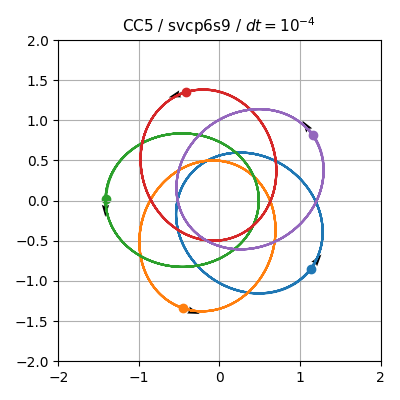
\includegraphics[width=.9\linewidth]{img/ccnmas5.png}
            \caption{Original}
        \end{figure}

    \column{.50\textwidth}\justifying
        \begin{figure}
            \centering
            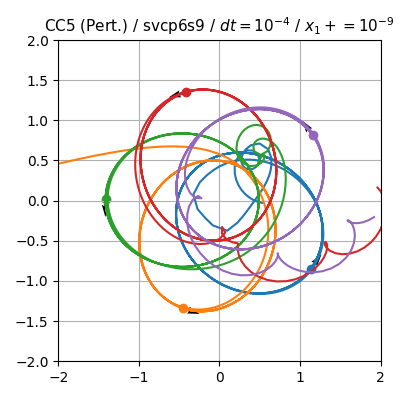
\includegraphics[width=.9\linewidth]{img/ccnmas5_pert.png}
            \caption{Perturbado ($10^{-9}$)}
        \end{figure}
\end{columns}

\end{frame}

%------------------------------------------------

\begin{frame}
\justifying
\frametitle{Faz sentido tudo isso? \cite[pp.234-240]{aarseth_gravitational_2003}}

% ADICIONAR EXEMPLO DE DUAS SIMULAÇÕES GRANDES DE MESMO VI COM MÉTODOS DIFERENTES

\begin{itemize}
    \item Estatisticamente, faz sim! 
    \item Trajetórias individuais podem não ser numericamente confiáveis...
    \item Mas a solução numérica não necessariamente é inválida!
    \item Shadow orbits... \cite{shadoworbits}
\end{itemize}

\end{frame}

%------------------------------------------------

\begin{frame}
\justifying
\frametitle{Exemplo}

{\color{blue}\href{https://ime.usp.br/~oapotalej/arquivos/coloquinho2026/exemplo_700.html}{Exemplo com 700 corpos.}}

\begin{columns}
    \column{.50\textwidth}\justifying
        \begin{figure}
            \centering
            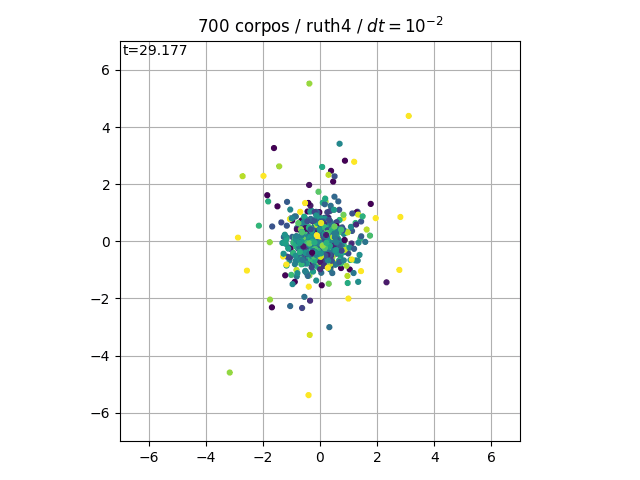
\includegraphics[width=.9\linewidth]{img/estatisticas/700corpos_ruth4.png}
            \caption{Integrado com Ruth4}
        \end{figure}
    \column{.50\textwidth}\justifying
        \begin{figure}
            \centering
            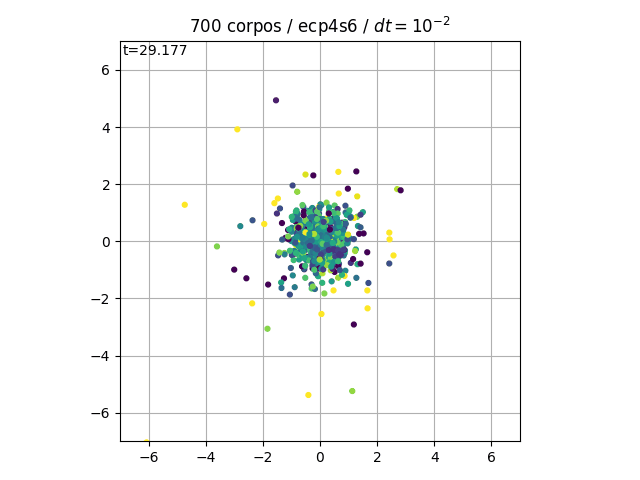
\includegraphics[width=.9\linewidth]{img/estatisticas/700corpos_ecp4s6.png}
            \caption{Integrado com ecp4s6}
        \end{figure}
\end{columns}

\end{frame}

%------------------------------------------------

\begin{frame}
\justifying
\frametitle{Exemplo}

\begin{itemize}
    \item O sistema cresce quase do mesmo jeito em ambos os casos...
\end{itemize}

\begin{columns}
    \column{.5\textwidth}\justifying
        \begin{figure}
            \centering
            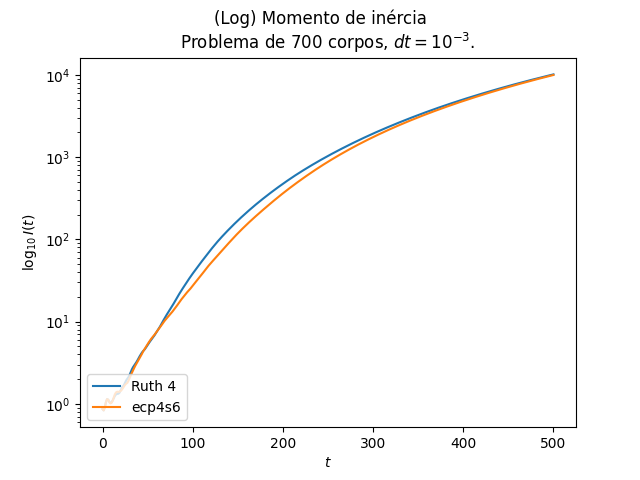
\includegraphics[width=.9\linewidth]{img/estatisticas/700_inercia.png}
            \caption{Inércia}
        \end{figure}
    \column{.5\textwidth}\justifying
        \begin{figure}
            \centering
            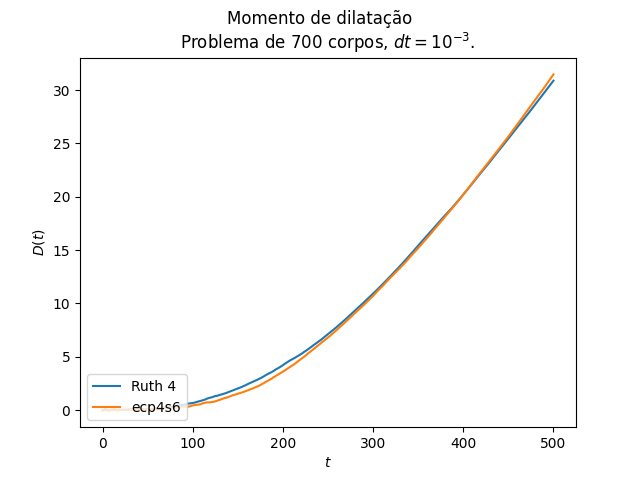
\includegraphics[width=.9\linewidth]{img/estatisticas/700_dilatacao.png}
            \caption{Dilatação}
        \end{figure}
\end{columns}

\end{frame}

%------------------------------------------------

\begin{frame}
\justifying
\frametitle{Exemplo}

\begin{itemize}
    \item O sistema cresce quase do mesmo jeito em ambos os casos...
\end{itemize}

\begin{columns}
    \column{.5\textwidth}\justifying
        \begin{figure}
            \centering
            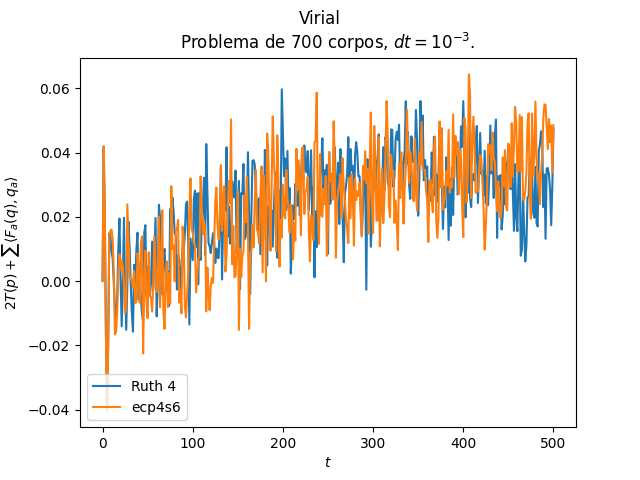
\includegraphics[width=.9\linewidth]{img/estatisticas/700_virial.png}
            \caption{Virial}
        \end{figure}
    \column{.5\textwidth}\justifying
        \begin{figure}
            \centering
            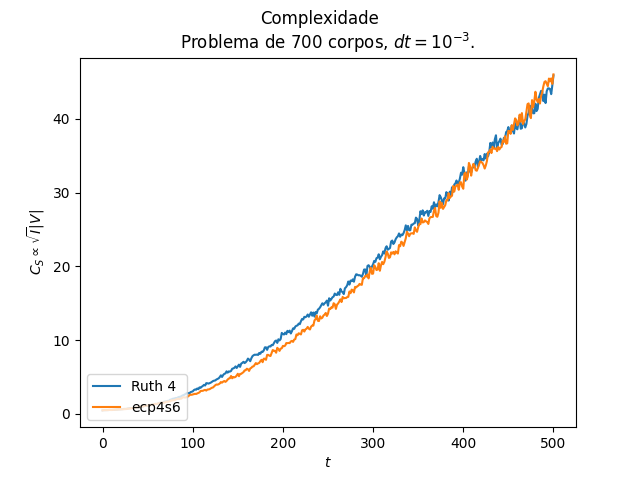
\includegraphics[width=.9\linewidth]{img/estatisticas/700_complexidade.png}
            \caption{Complexidade}
        \end{figure}
\end{columns}

\end{frame}

% %------------------------------------------------

% \begin{frame}
% \justifying
% \frametitle{O que estou estudando}

% [Falar sobre a dinâmica]

% \end{frame}

% %------------------------------------------------

\begin{frame}
\justifying
\frametitle{Outras possibilidades...}

\begin{columns}[c]
\column{.55\textwidth}\justifying
    \begin{itemize}
        \item Outros métodos/formas:
        \begin{itemize}
            \item Implícitos;
            \item Variacionais;
            \item Exatos;
            \item Tamanho de passo variável...
        \end{itemize}
        
        \item Específicos:
        \begin{itemize}
            \item Tamanhos de passo individuais;
            \item \textit{block-timesteps};
            \item Esquemas hierárquicos;
            \item Wisdom-Holman (Sistema solar);
            \item Barnes-Hut, \textit{Particle-Mesh}, SPH...
        \end{itemize}
        
        \item \textit{Ao infinito e além!}
    \end{itemize}
    
\column{.45\textwidth}\justifying
    \begin{figure}
        \centering
        \begin{subfigure}[b]{0.47\textwidth}
            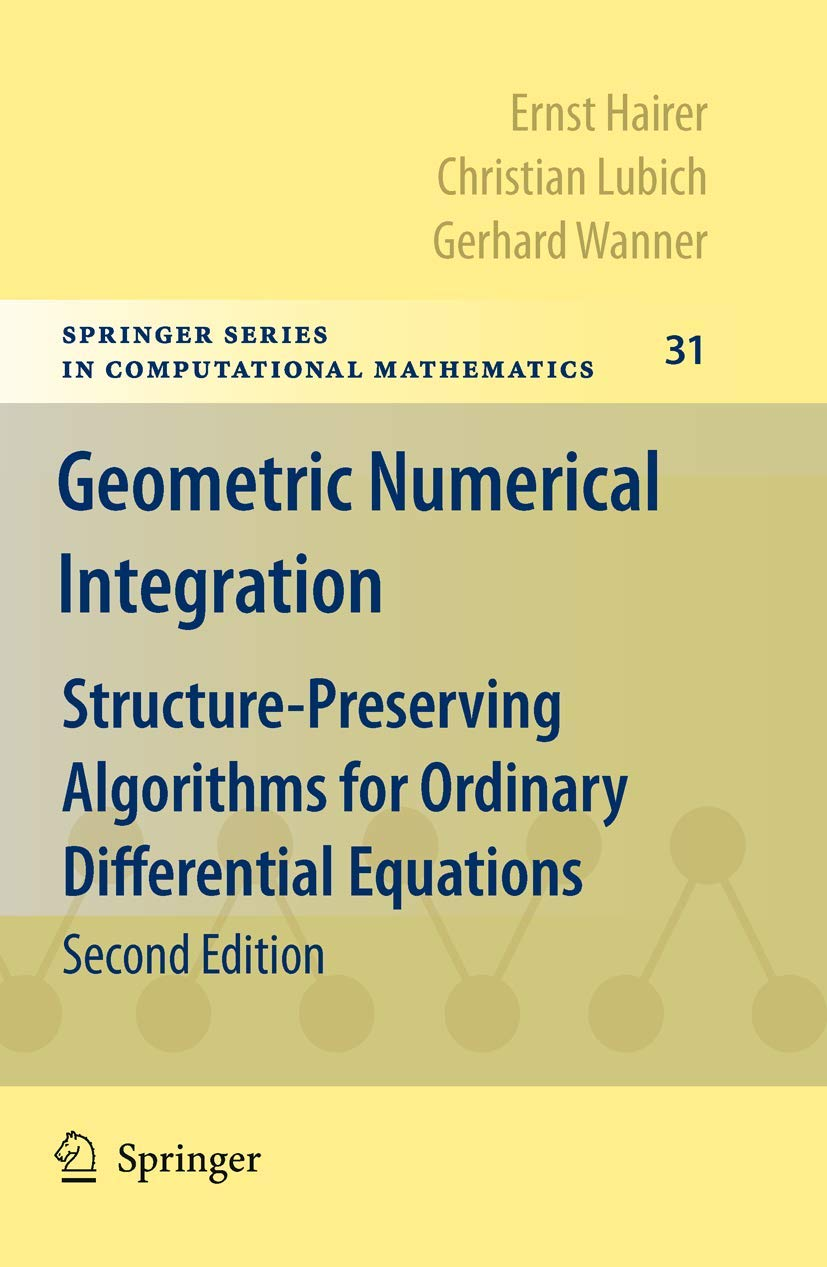
\includegraphics[width=\linewidth]{img/hairer.jpg}
        \end{subfigure}
        \hfill
        \begin{subfigure}[b]{0.47\textwidth}
            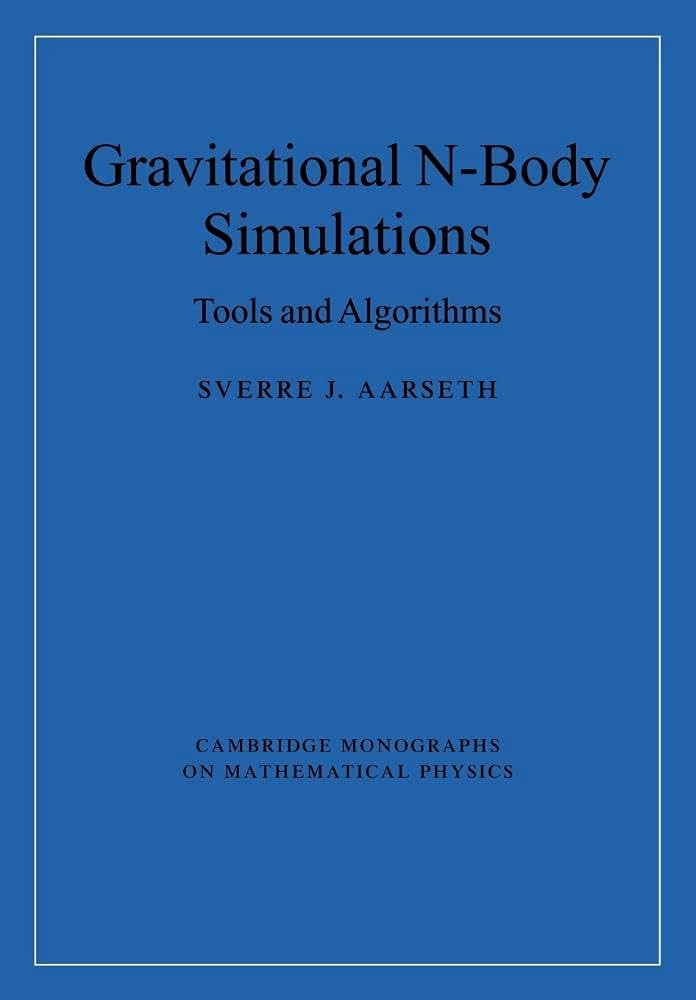
\includegraphics[width=\linewidth]{img/aarseth.jpg}
        \end{subfigure}
    \end{figure}
\end{columns}

\end{frame}

%------------------------------------------------

\begin{frame}
\justifying
\frametitle{Conclusão}

\begin{figure}
    \centering
    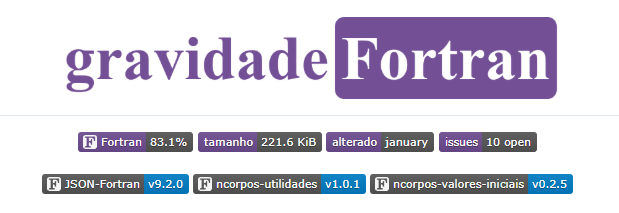
\includegraphics[width=0.7\linewidth]{img/gf-logo.png}
    \caption{\href{https://github.com/potalej/gravidade-fortran}{https://github.com/potalej/gravidade-fortran}}
\end{figure}

\begin{itemize}
    \item O PNCG é muito amplo, problemas específicos são melhor resolvidos com soluções específicas. ``Meus N-corpos, minhas regras.''
\end{itemize}

\end{frame}

%------------------------------------------------

\begin{frame}[plain]
  \centering
  \vspace{0.5cm}
  \Huge Obrigado!
\end{frame}

%------------------------------------------------